\documentclass[tikz,border=10pt]{standalone}
\usepackage{tikz}
\usepackage{amsmath}
\usepackage{xcolor}
\usetikzlibrary{shapes,arrows,positioning,calc}

% Define colors
\definecolor{culture1}{RGB}{220, 20, 60}      % Western/Individualistic 
\definecolor{culture2}{RGB}{30, 144, 255}     % Eastern/Collectivist
\definecolor{culture3}{RGB}{255, 140, 0}      % African/Ubuntu
\definecolor{culture4}{RGB}{50, 205, 50}      % Nordic/Social Democratic
\definecolor{adaptation}{RGB}{138, 43, 226}   % Adaptation engine
\definecolor{universal}{RGB}{255, 215, 0}     % Universal principles
\definecolor{background}{RGB}{248, 249, 250}

\begin{document}
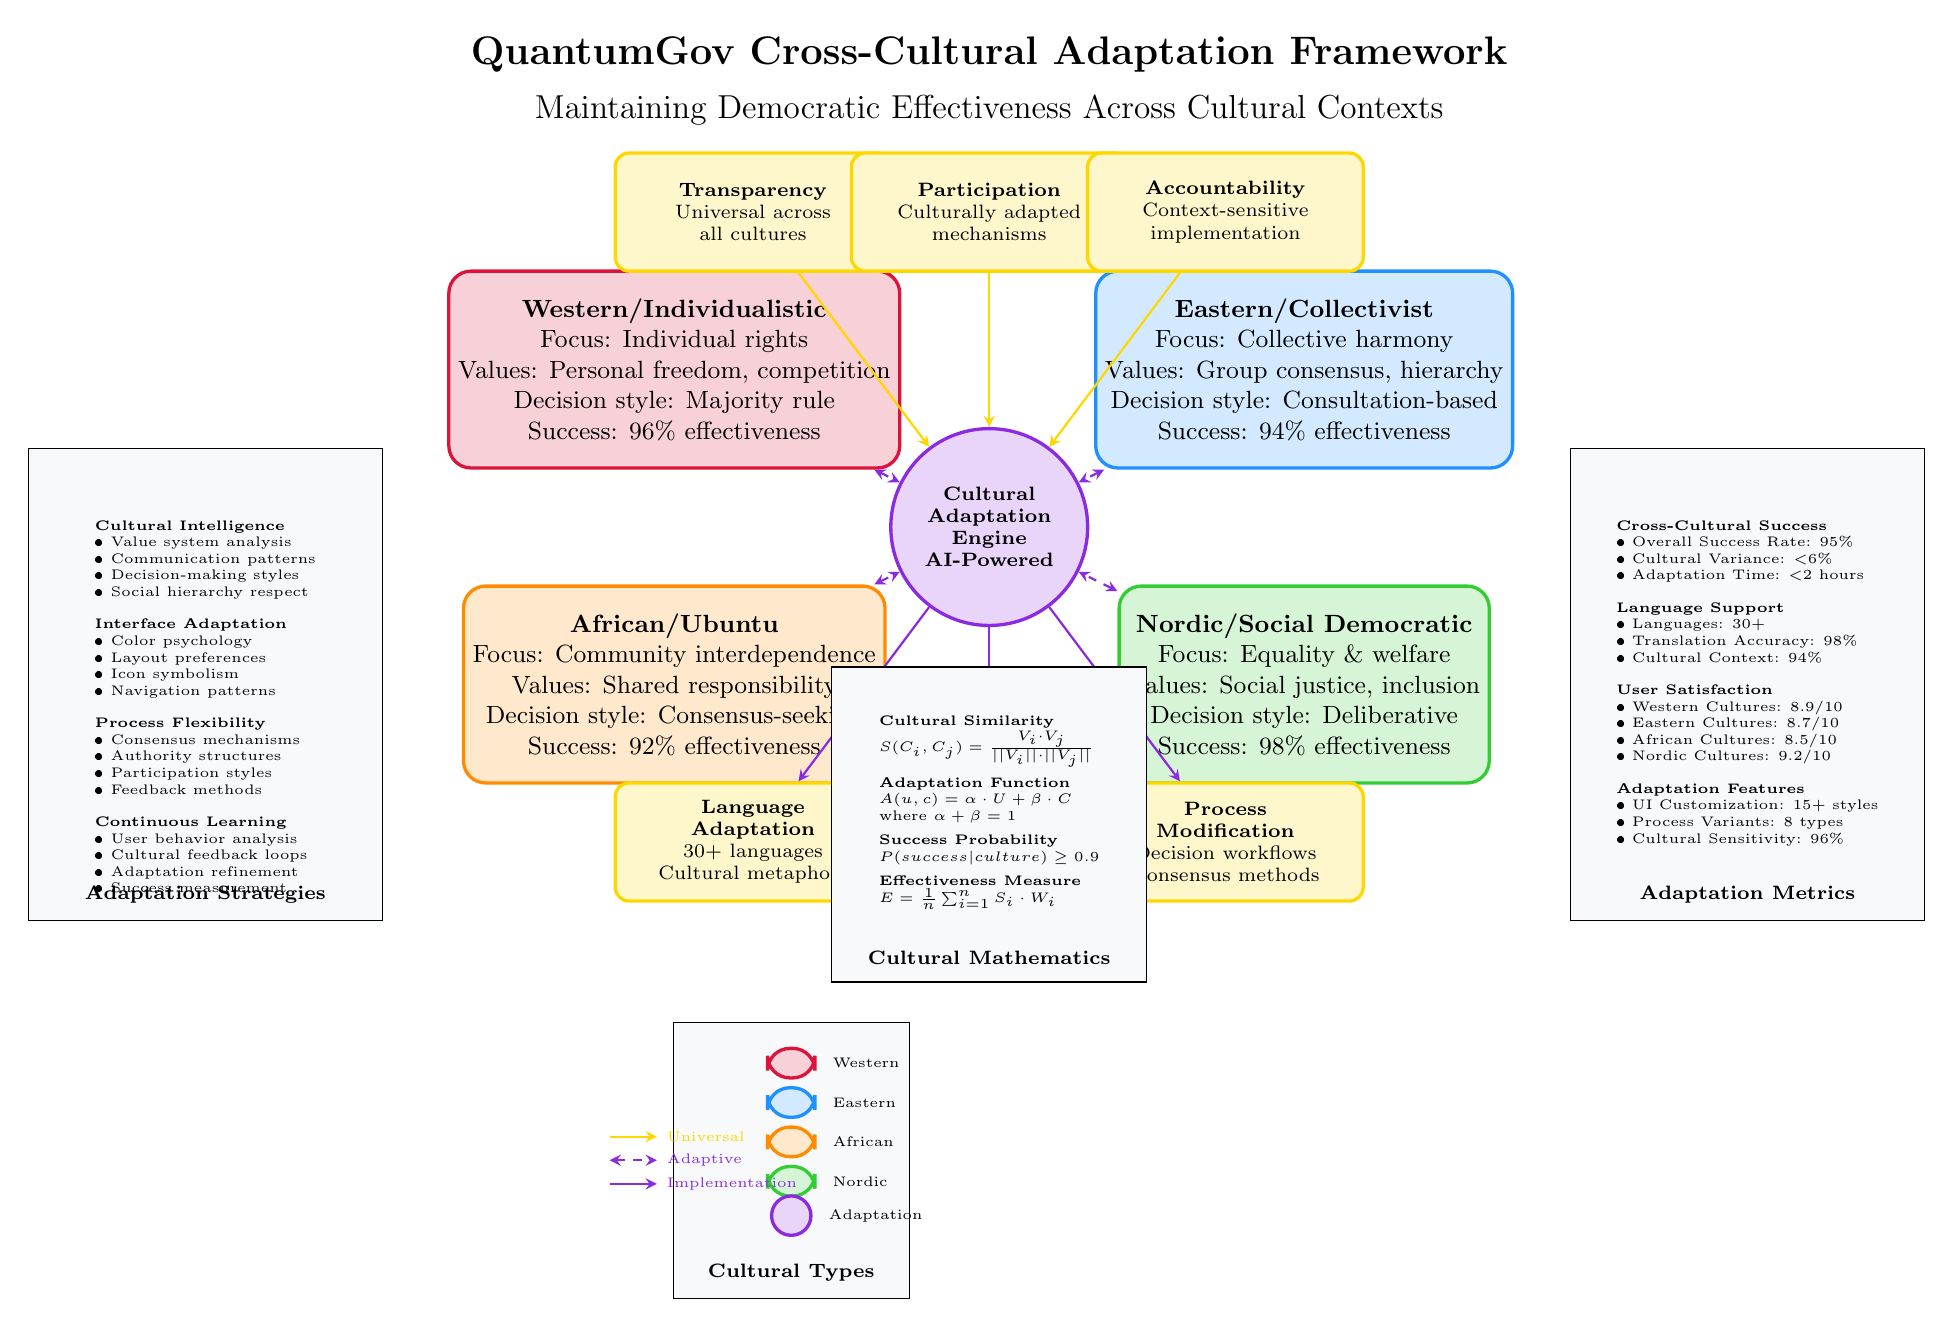
\begin{tikzpicture}[
    node distance=1.5cm,
    culture_box/.style={rectangle, rounded corners=8pt, draw, minimum height=2.5cm, minimum width=4cm, align=center, font=\small, very thick},
    adaptation_node/.style={circle, draw=adaptation, fill=adaptation!20, minimum size=2.5cm, align=center, font=\scriptsize, very thick},
    universal_box/.style={rectangle, rounded corners=5pt, draw=universal, fill=universal!20, minimum height=1.5cm, minimum width=3.5cm, align=center, font=\scriptsize, very thick},
    flowline/.style={->, thick, >=stealth},
    adaptive/.style={<->, thick, >=stealth, color=adaptation, dashed}
]

% Title
\node[align=center, font=\Large\bfseries] at (0, 12) {QuantumGov Cross-Cultural Adaptation Framework};
\node[align=center, font=\large] at (0, 11.3) {Maintaining Democratic Effectiveness Across Cultural Contexts};

% Cultural Contexts (arranged in a circle)
\node[culture_box, draw=culture1, fill=culture1!20] (western) at (-4, 8) {
    \textbf{Western/Individualistic}\\
    Focus: Individual rights\\
    Values: Personal freedom, competition\\
    Decision style: Majority rule\\
    Success: 96\% effectiveness
};

\node[culture_box, draw=culture2, fill=culture2!20] (eastern) at (4, 8) {
    \textbf{Eastern/Collectivist}\\
    Focus: Collective harmony\\
    Values: Group consensus, hierarchy\\
    Decision style: Consultation-based\\
    Success: 94\% effectiveness
};

\node[culture_box, draw=culture3, fill=culture3!20] (african) at (-4, 4) {
    \textbf{African/Ubuntu}\\
    Focus: Community interdependence\\
    Values: Shared responsibility\\
    Decision style: Consensus-seeking\\
    Success: 92\% effectiveness
};

\node[culture_box, draw=culture4, fill=culture4!20] (nordic) at (4, 4) {
    \textbf{Nordic/Social Democratic}\\
    Focus: Equality \& welfare\\
    Values: Social justice, inclusion\\
    Decision style: Deliberative\\
    Success: 98\% effectiveness
};

% Central Adaptation Engine
\node[adaptation_node] (adaptation_core) at (0, 6) {
    \textbf{Cultural}\\
    \textbf{Adaptation}\\
    \textbf{Engine}\\
    \textbf{AI-Powered}
};

% Universal Principles (Top)
\node[universal_box] (transparency) at (-3, 10) {
    \textbf{Transparency}\\
    Universal across\\
    all cultures
};

\node[universal_box] (participation) at (0, 10) {
    \textbf{Participation}\\
    Culturally adapted\\
    mechanisms
};

\node[universal_box] (accountability) at (3, 10) {
    \textbf{Accountability}\\
    Context-sensitive\\
    implementation
};

% Adaptation Mechanisms (Bottom)
\node[universal_box] (language) at (-3, 2) {
    \textbf{Language}\\
    \textbf{Adaptation}\\
    30+ languages\\
    Cultural metaphors
};

\node[universal_box] (interface) at (0, 2) {
    \textbf{Interface}\\
    \textbf{Customization}\\
    Cultural UI patterns\\
    Visual preferences
};

\node[universal_box] (process) at (3, 2) {
    \textbf{Process}\\
    \textbf{Modification}\\
    Decision workflows\\
    Consensus methods
};

% Connections from cultures to adaptation core
\draw[adaptive] (western) -- (adaptation_core);
\draw[adaptive] (eastern) -- (adaptation_core);
\draw[adaptive] (african) -- (adaptation_core);
\draw[adaptive] (nordic) -- (adaptation_core);

% Connections from universal principles to adaptation core
\draw[flowline, color=universal] (transparency) -- (adaptation_core);
\draw[flowline, color=universal] (participation) -- (adaptation_core);
\draw[flowline, color=universal] (accountability) -- (adaptation_core);

% Connections from adaptation core to mechanisms
\draw[flowline, color=adaptation] (adaptation_core) -- (language);
\draw[flowline, color=adaptation] (adaptation_core) -- (interface);
\draw[flowline, color=adaptation] (adaptation_core) -- (process);

% Performance metrics panel
\node[draw, fill=background, minimum width=4.5cm, minimum height=6cm, right=1cm of nordic] (metrics) {};
\node[above=0.1cm of metrics.south, font=\scriptsize\bfseries, align=center] {Adaptation Metrics};
\node[below=0.8cm of metrics.north, font=\tiny, align=left] {
    \textbf{Cross-Cultural Success}\\
    • Overall Success Rate: 95\%\\
    • Cultural Variance: <6\%\\
    • Adaptation Time: <2 hours\\[0.2cm]
    \textbf{Language Support}\\
    • Languages: 30+\\
    • Translation Accuracy: 98\%\\
    • Cultural Context: 94\%\\[0.2cm]
    \textbf{User Satisfaction}\\
    • Western Cultures: 8.9/10\\
    • Eastern Cultures: 8.7/10\\
    • African Cultures: 8.5/10\\
    • Nordic Cultures: 9.2/10\\[0.2cm]
    \textbf{Adaptation Features}\\
    • UI Customization: 15+ styles\\
    • Process Variants: 8 types\\
    • Cultural Sensitivity: 96\%
};

% Adaptation strategies panel
\node[draw, fill=background, minimum width=4.5cm, minimum height=6cm, left=1cm of african] (strategies) {};
\node[above=0.1cm of strategies.south, font=\scriptsize\bfseries, align=center] {Adaptation Strategies};
\node[below=0.8cm of strategies.north, font=\tiny, align=left] {
    \textbf{Cultural Intelligence}\\
    • Value system analysis\\
    • Communication patterns\\
    • Decision-making styles\\
    • Social hierarchy respect\\[0.2cm]
    \textbf{Interface Adaptation}\\
    • Color psychology\\
    • Layout preferences\\
    • Icon symbolism\\
    • Navigation patterns\\[0.2cm]
    \textbf{Process Flexibility}\\
    • Consensus mechanisms\\
    • Authority structures\\
    • Participation styles\\
    • Feedback methods\\[0.2cm]
    \textbf{Continuous Learning}\\
    • User behavior analysis\\
    • Cultural feedback loops\\
    • Adaptation refinement\\
    • Success measurement
};

% Mathematical framework
\node[draw, fill=background, minimum width=4cm, minimum height=4cm, below=0.5cm of adaptation_core] (math_framework) {};
\node[above=0.1cm of math_framework.south, font=\scriptsize\bfseries, align=center] {Cultural Mathematics};
\node[below=0.5cm of math_framework.north, font=\tiny, align=left] {
    \textbf{Cultural Similarity}\\
    $S(C_i, C_j) = \frac{V_i \cdot V_j}{||V_i|| \cdot ||V_j||}$\\[0.1cm]
    \textbf{Adaptation Function}\\
    $A(u, c) = \alpha \cdot U + \beta \cdot C$\\
    where $\alpha + \beta = 1$\\[0.1cm]
    \textbf{Success Probability}\\
    $P(success|culture) \geq 0.9$\\[0.1cm]
    \textbf{Effectiveness Measure}\\
    $E = \frac{1}{n}\sum_{i=1}^n S_i \cdot W_i$
};

% Legend
\node[draw, fill=background, minimum width=3cm, minimum height=3.5cm, below left=0.5cm and -1cm of math_framework] (legend) {};
\node[above=0.1cm of legend.south, font=\scriptsize\bfseries, align=center] {Cultural Types};
\node[culture_box, scale=0.15, draw=culture1, fill=culture1!20, above=2.8cm of legend.south] (leg_western) {};
\node[right=0.1cm of leg_western, font=\tiny] {Western};
\node[culture_box, scale=0.15, draw=culture2, fill=culture2!20, above=2.3cm of legend.south] (leg_eastern) {};
\node[right=0.1cm of leg_eastern, font=\tiny] {Eastern};
\node[culture_box, scale=0.15, draw=culture3, fill=culture3!20, above=1.8cm of legend.south] (leg_african) {};
\node[right=0.1cm of leg_african, font=\tiny] {African};
\node[culture_box, scale=0.15, draw=culture4, fill=culture4!20, above=1.3cm of legend.south] (leg_nordic) {};
\node[right=0.1cm of leg_nordic, font=\tiny] {Nordic};
\node[adaptation_node, scale=0.2, above=0.8cm of legend.south] (leg_adapt) {};
\node[right=0.1cm of leg_adapt, font=\tiny] {Adaptation};

% Flow Legend
\draw[flowline, color=universal] (legend.west) ++(-0.8, 0.3) -- ++(0.6, 0) node[right, font=\tiny] {Universal};
\draw[adaptive] (legend.west) ++(-0.8, 0) -- ++(0.6, 0) node[right, font=\tiny] {Adaptive};
\draw[flowline, color=adaptation] (legend.west) ++(-0.8, -0.3) -- ++(0.6, 0) node[right, font=\tiny] {Implementation};

\end{tikzpicture}
\end{document}